\documentclass{article}
\usepackage{graphicx} % Required for inserting images
\usepackage[top=0.9in, bottom=1in, left=1.5in, right=1.5in]{geometry}
\usepackage[utf8]{inputenc}
\usepackage[icelandic]{babel}
\usepackage[T1]{fontenc}
\usepackage[sc]{mathpazo}
\usepackage[parfill]{parskip}
\renewcommand{\baselinestretch}{1.2}
% Tables and lists
\usepackage{booktabs,tabularx}
\usepackage{multirow}
\usepackage{enumerate}
\usepackage{adjustbox}
\usepackage{multicol}
\usepackage{xcolor}
\usepackage{algpseudocode}
\usepackage{tikz}
\usepackage{nicefrac}
\usepackage{changepage}
\usepackage{fancyvrb}
\usetikzlibrary{arrows, positioning, calc, graphs}

% Math
\usepackage{amsmath, amsfonts, amssymb, amsthm}
% Graphics

\usepackage{graphicx}
\usepackage{tikz}
% Code environment
\usepackage{minted}
%\usepackage{bm}
%\usepackage{siunitx}
%\usepackage{animate}
%\usepackage{hyperref}
%\usepackage{movie15}
%\usepackage{multicol}
%\usepackage{changepage}
\title{Forritunarmál Einstaklingsverkefni 3}
\author{Ragnar Björn Ingvarsson, rbi3}
\tikzset{->, >=stealth', shorten >=1pt, node distance=2cm,thick, main node/.style={circle,draw,minimum size=3em}}


\begin{document}
\renewcommand\thepage{}
	
	\maketitle

	\newpage
	\setcounter{page}{1}
	\renewcommand\thepage{\arabic{page}}

	\section{$\lambda x.((x + z) / z)$}
	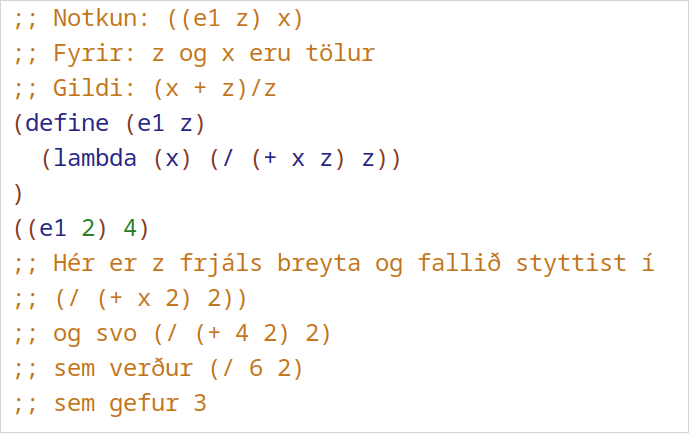
\includegraphics[scale=0.3]{e1.png}

	Við skrifum þetta í Scheme sem \texttt{(lambda (x) (/ (+ x z) z))}. 
	Segðin skilar falli sem er með frjálsu breytuna $z$. Fallið virkar 
	þannig að það tekur inn eitt inntak, x, og skilar $\frac{x + z}{z}$.

	Við getum til dæmis sagt í Scheme

	\begin{verbatim}
(define (e1 z)
	(lambda (x) (/ (+ x z) z))
)
((e1 2) 4)
	\end{verbatim}

	Sem skilar $3$.

	\begin{center}
		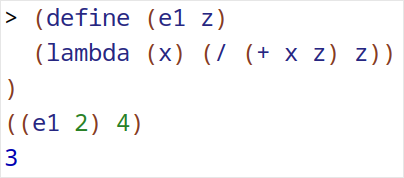
\includegraphics[scale=0.375]{z.png}
	\end{center}

	Síðan getum við endurskrifað segðina með öðrum táknum sem:

	\[\lambda a.((a + b)/b)\]

	Eða í Scheme:

	\begin{center}\texttt{(lambda (a) (/ (+ a b) b))}\end{center}

	\section{$\lambda x.(\lambda y.(\lambda z.x(y(yz))))$}

	\begin{center}
		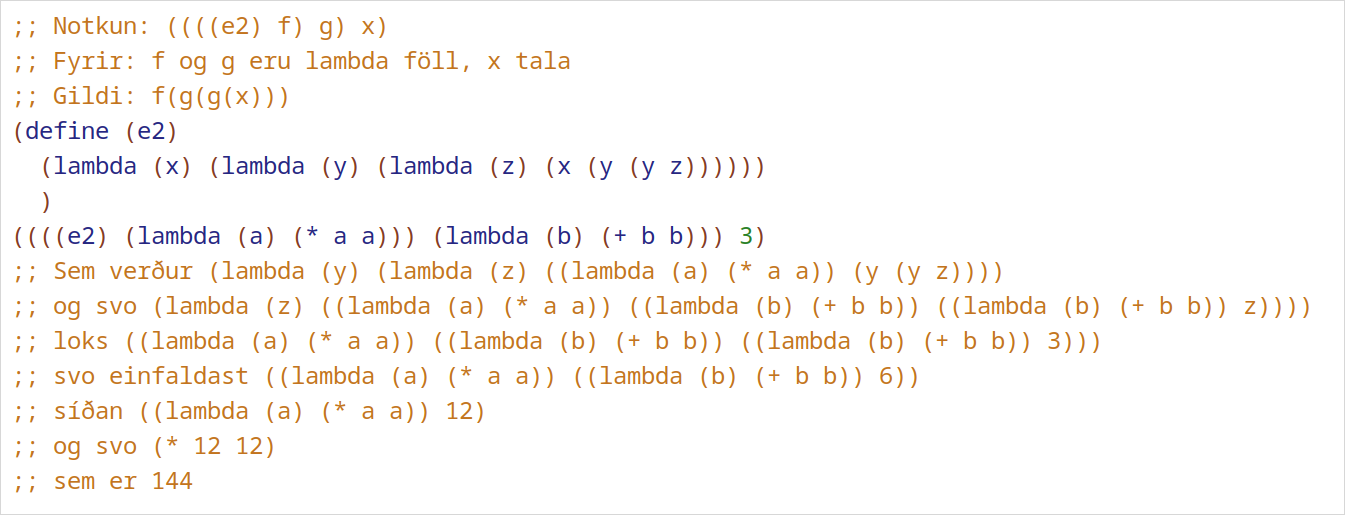
\includegraphics[scale=0.3]{e2.png}
	\end{center}

	Þetta myndi vera í Scheme: \texttt{(lambda (x) (lambda (y) (lambda (z) 
	(x (y (y z))))))}. Segðin skilar falli sem virkar svo að það tekur inn 
	þrjú inntök, tvö föll, $f$ og $g$, og eitt gildi, $x$. 
	Síðan skilar það niðurstöðunni úr $f(g(g(x)))$

	Hér er engin frjáls breyta en við getum notað fallið til dæmis svo:

	\begin{verbatim}
(define (e2)
	(lambda (x) (lambda (y) (lambda (z) (x (y (y z))))))
	)
((((e2) (lambda (a) (* a a))) (lambda (b) (+ b b))) 3)
	\end{verbatim}

	Þar sem við segjum að $f(x) = x^2$ og $g(x) = 2x$ og gefum því $x=3$. 
	Því fáum við sem niðurstöðu einfalda gildið $144$.

	\begin{center}
		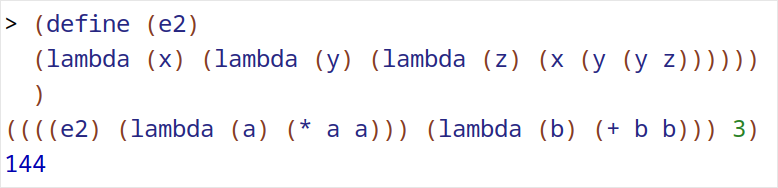
\includegraphics[scale=0.275]{144.png}
	\end{center}

	Við getum svo endurskrifað segðina með öðrum táknum sem:

	\[\lambda a.(\lambda b.(\lambda c.a(b(bc))))\]

	Eða í Scheme:

	\begin{center}\texttt{(lambda (a) (lambda (b) 
	(lambda (c) (a (b (b c))))))}\end{center}

\end{document}
